\documentclass[a4paper,10pt]{article}
\usepackage[utf8]{inputenc}
\usepackage[spanish]{babel}
\usepackage[affil-it]{authblk}
\usepackage{enumerate}
\usepackage{graphicx}
\usepackage{hyperref}
\usepackage{amsmath}
\usepackage{amssymb}
\usepackage{cancel}
\usepackage[usenames, dvipsnames]{color}
\usepackage{tikz}
\usepackage{multimedia}
\usepackage{subcaption} %Multiple images
\usepackage{multicol} % Multiple columns
\usepackage{float}
\usepackage{cleveref}
\usepackage[margin=1.4in]{geometry}
\usepackage[labelfont=bf]{caption}
\usetikzlibrary{calc}
\numberwithin{equation}{section}

%Columns separation
\setlength{\columnsep}{1cm}

%Indentation
\setlength{\parindent}{0ex}

%Multiple References

\usepackage{xparse}
\ExplSyntaxOn
\NewDocumentCommand{\mref}{m}{\quinn_mref:n {#1}}
\seq_new:N \l_quinn_mref_seq
\cs_new:Npn \quinn_mref:n #1
 {
  \seq_set_split:Nnn \l_quinn_mref_seq { , } { #1 }
  \seq_pop_right:NN \l_quinn_mref_seq \l_tmpa_tl
  ( % print the left parenthesis
  \seq_map_inline:Nn \l_quinn_mref_seq
    { \ref{##1},\nobreakspace } % print the first references
  \exp_args:NV \ref \l_tmpa_tl 
  ) 
 }
\ExplSyntaxOff


%Boxes

\newcommand*{\boxcolor}{blue}
\makeatletter
\renewcommand{\boxed}[1]{\textcolor{\boxcolor}{%
\tikz[baseline={([yshift=-1ex]current bounding box.center)}] \node [rectangle, minimum width=1ex,rounded corners,draw] {\normalcolor\m@th$\displaystyle#1$};}}
 \makeatother

%Constantes
\newcommand{\euler}{\mathrm{e}}
\newcommand{\im}{i}

%Lemas, teoremas, definiciones y pruebas
\newcommand{\definicion}{\textbf{Definición: }}
\newcommand{\lema}{\textbf{Lema: }}
\newcommand{\teorema}{\textbf{Teorema: }}
\newcommand{\prueba}{\textbf{Prueba: }}


%opening
\title{Mecánica Clásica Tarea \# 6}
\author{Favio Vázquez\thanks{Correo: favio.vazquezp@gmail.com}}\affil{Instituto de Ciencias Nucleares. Universidad Nacional Autónoma de México.}
\date{}

\begin{document}

\makeatletter
\def\@maketitle{%
  \newpage
  \null
  \vskip 2em%
  \begin{center}%
  \let \footnote \thanks
    {\Large\bfseries \@title \par}%
    \vskip 1.5em%
    {\normalsize
      \lineskip .5em%
      \begin{tabular}[t]{c}%
        \@author
      \end{tabular}\par}%
    \vskip 1em%
    {\normalsize \@date}%
  \end{center}%
  \par
  \vskip 1.5em}
\makeatother

\maketitle

\section{Problema 1}

Una partícula de masa $m$ se mueve constreñida a la superficie de un paraboloide de 
revolución que tiene su abertura hacia arriba en presencia del campo de la gravedad. 
Calcule las fuerzas de constricción.

\vspace{.3cm}

\underline{Solución:} \vspace{.3cm}

Para visualizar mejor el problema al cual nos enfrentamos, se muestra en la figura 
de abajo una partícula de masa $m$ constreñida a moverse en dicho paraboloide.

\begin{figure}[H]
 \center 
 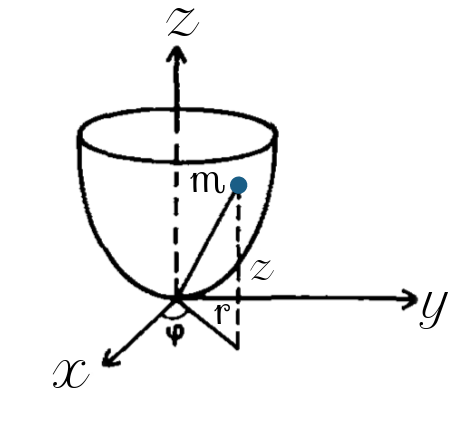
\includegraphics[scale=0.5]{problema1fig1}
 \caption{Partícula de masa $m$ se mueve constreñida a la superficie de un paraboloide de 
revolución}
\label{fig:problema1fig1}
\end{figure}

Debido a las simetrías involucradas en este problema, utilizaremos coordenadas cilíndricas 
polares para resolverlo. Tenemos entonces las siguientes transformaciones de coordenadas,

\begin{align}
 x &= r\cos{\phi}, \\
 y &= r\sen{\phi}, \\
 z &= z.
 \label{eq:transfCoordenadasParab}
\end{align}

Por otra parte, tenemos la constricción holonómica de que la partícula debe moverse 
en la superficie del paraboloide de revolución, que podemos expresar como

\begin{equation}
 x^2 + y^2 = \alpha z.
\end{equation}

Pero en las coordenadas que estamos utilizando

\begin{equation}
 x^2 + y^2 = r^2,
\end{equation}

entonces la constricción se convierte en,

\begin{equation}
 \xi(r,\phi,z) \equiv - r^2 + \alpha z = 0.
 \label{eq:constriccionParab}
\end{equation}

Siguiendo la receta lagrangiana calculemos ahora la energía cinética y la potencial 
en nuestras coordenadas generalizadas $(r,\phi,z)$. Recordemos que podemos escribir 
estas energías en coordenadas cartesianas como,

\begin{equation}
 T = \frac{1}{2}m(\dot{x}^2 + \dot{y}^2 +\dot{z}^2).
 \label{eq:energCinetParab1}
\end{equation}

\begin{equation}
 V = mgz.
 \label{eq:energPotenParab1}
\end{equation}

Debido a que la partícula se encuentra en un campo gravitacional uniforme. Expresemos 
ahora estas energías en términos de nuestras coordenadas generalizadas. Cabe resaltar 
que utilizaremos el método de los multiplicadores indeterminados de Lagrange para obtener 
las fuerzas generalizadas, por lo cual haremos uso de la constricción en los momentos 
indicados por esta metodología. 

\vspace{.3cm}

Comencemos por obtener las derivadas temporales de \mref{eq:transfCoordenadasParab}, 
para introducirlas en \mref{eq:energCinetParab1},

\begin{align}
 \dot{x} &= \dot{r}\cos{\phi} - r \dot{\phi}\sen{\phi}, \\
 \dot{y} &= \dot{r}\sen{\phi} + r \dot{\phi}\cos{\phi}, \\
 \dot{z} &= \dot{z}.
 \label{eq:derivTemprTransfCoordParab}
\end{align}

Introduciendo \mref{eq:derivTemprTransfCoordParab} en \mref{eq:energCinetParab1} obtenemos,

\begin{align}
 \begin{split}
  T &= \frac{1}{2}m [( \dot{r}\cos{\phi} - r \dot{\phi}\sen{\phi})^2
  + (\dot{r}\sen{\phi} + r \dot{\phi}\cos{\phi})^2 + \dot{z}^2], \\
  %  
  &= \frac{1}{2} m (\dot{r}^2\cos^2{\phi} - \cancel{2r\dot{r}\dot{\phi}\cos{\phi}\sen{\phi}} + 
  r^2\dot{\phi}^2 \sen^2{\phi} +  \dot{r}^2\sen^2{\phi} \\
  %
  &+ \cancel{2r\dot{r}\dot{\phi}\cos{\phi}\sen{\phi}}
  + r^2\dot{\phi}^2 \cos^2{\phi} + \dot{z}^2 ) \\
  %
  &= \frac{1}{2} m \left[ \dot{r}^2\cancelto{1}{(\sen^2{\phi} + \cos^2{\phi})}
  + r^2\dot{\phi}^2 \cancelto{1}{(\sen^2{\phi} + \cos^2{\phi})} + \dot{z}^2 \right]
  %%
 \end{split}
\end{align}

\begin{equation}
 \therefore T = \frac{1}{2}m(\dot{r}^2 + r^2\dot{\phi}^2 + \dot{z}^2).
 \label{eq:energCinetParab2}
\end{equation}

Entonces la lagrangiana del sistema sería

\begin{equation}
 L = \frac{1}{2} m(\dot{r}^2 + r^2\dot{\phi}^2 + \dot{z}^2) - mgz.
\end{equation}

Ahora utilizando el hecho de que las ecuaciones de Lagrange en la metodología de 
multiplicadores indeterminados, se convierten en,

\begin{equation}
  \frac{d}{dt}\frac{\partial L}{\partial \dot{q}^j} - \frac{\partial L}{\partial q^j}  
 - \sum_k \lambda_k(t) \frac{\partial \xi_k}{\partial q^j} = 0,
\end{equation}

y que las fuerzas generalizadas de constricción se encuentran con

\begin{equation}
 Q_j = \sum_k \lambda_k(t) \frac{\partial \xi_k}{\partial q^j}.
 \label{eq:fuerzasConstri1}
\end{equation}

estamos en posición para aplicar el método y obtener estas fuerzas. Tendremos entonces 
las siguientes ecuaciones para $r$, $z$ y $\phi$

\begin{equation}
 \frac{d}{dt}\frac{\partial L}{\partial \dot{r}} - \frac{\partial L}{\partial r}
 - \lambda \frac{\partial \xi}{\partial r} = 0,
\end{equation}

\begin{equation}
 \frac{d}{dt}\frac{\partial L}{\partial \dot{z}} - \frac{\partial L}{\partial z}
 - \lambda \frac{\partial \xi}{\partial z} = 0,
\end{equation}

\begin{equation}
 \frac{d}{dt}\frac{\partial L}{\partial \dot{\phi}} - \frac{\partial L}{\partial \phi}
 - \lambda \frac{\partial \xi}{\partial \phi} = 0.
\end{equation}

Entonces tenemos para $r$,

\begin{equation}
  \frac{d}{dt}(m\dot{r}) - m r\dot{\phi}^2 + 2 r = 0,
\end{equation}

\begin{equation}
 \boxed{m(\ddot{r} - r\dot{\phi}^2) + 2 \lambda r = 0}.
 \label{eq:ecuMovimientoR}
\end{equation}

Para $z$,

\begin{equation}
 \frac{d}{dt}(m\dot{z}) + mg + \lambda \alpha = 0.
\end{equation}

\begin{equation}
 \boxed{m(\ddot{z}+g) + \lambda \alpha = 0 }.
 \label{eq:ecuMovimientoZ}
\end{equation}

Y para $\phi$,

\begin{equation}
 \frac{d}{dt}(mr^2\dot{\phi}) = 0.
\end{equation}

\begin{equation}
 \boxed{mr^2\dot{\phi} = \text{constante} = l}.
 \label{eq:ecuMovimientoPhi}
\end{equation}

Donde como puede verse debido a que $\phi$ es una coordenada cíclica, encontramos 
una integral de movimiento a la cual asociamos el momentum angular, el cual se 
conserva durante el movimiento de la partícula.

\vspace{.3cm}

Para poder hallar las fuerzas de constricción debemos encontrar un valor para 
$\lambda$, lo cual podemos hacer utilizando la ecuación para la constricción 
\mref{eq:constriccionParab} y vemos que 

\begin{equation}
 \alpha z = r^2,
\end{equation}

\begin{equation}
\alpha \dot{z} = 2r \dot{r},
\end{equation}

\begin{equation}
\alpha \ddot{z} = 2(\dot{r}^2 + r\ddot{r}),
\end{equation}

\begin{equation}
 \therefore \ddot{z} = 2 \frac{(\dot{r}^2 + r\ddot{r})}{\alpha}.
 \label{eq:derivConstriccionParab}
\end{equation}

Pero por la ecuación \mref{eq:ecuMovimientoZ} y usando \mref{eq:derivConstriccionParab}
vemos que,

\begin{equation}
 \ddot{z} = 2 \frac{(\dot{r}^2 + r\ddot{r})}{\alpha} = - \frac{\lambda \alpha}{m} - g,
\end{equation}

entonces,

\begin{equation}
 \ddot{r} = - \frac{\lambda \alpha^2}{2mr} - \frac{g\alpha}{2r} - \frac{\dot{r}^2}{r}.
\label{eq:doblederivR}
\end{equation}

Ahora sustituyendo \mref{eq:doblederivR} en \mref{eq:ecuMovimientoR}, y utilizando 
el hecho que $\dot{\phi}^2 = l^2/m^2r^4$ obtenemos

\begin{equation}
 m(- \frac{\lambda \alpha^2}{2mr} - \frac{g\alpha}{2r} - \frac{\dot{r}^2}{r}.
 - \frac{l^2}{m^2r^3}) + 2\lambda r = 0.
\end{equation}

Reescribiendo y agrupando términos de $\lambda$ vemos que

\begin{equation}
 - \frac{\lambda \alpha^2}{2r} + 2 \lambda r = \frac{gm\alpha}{2r} + \frac{2m\dot{r}^2}{r},
 - \frac{l^2}{mr^3}
\end{equation}

\begin{equation}
 \lambda \left(2r - \frac{\alpha^2}{2r}\right) = \frac{gm\alpha}{2r} + \frac{2m\dot{r}^2}{r},
 - \frac{l^2}{mr^3}
\end{equation}

\begin{equation}
 \lambda \left(\frac{4r^2 - \alpha^2}{2r}\right) = \frac{gm\alpha}{2r} + \frac{2m\dot{r}^2}{r},
 - \frac{l^2}{mr^3}
\end{equation}

\begin{equation}
 \lambda(4r^2 - \alpha^2) = gm\alpha + 4 m\dot{r}^2 - \frac{2l^2}{mr^2},
\end{equation}

\begin{equation}
 \boxed{\lambda = \frac{1}{4r^2 - \alpha^2} \left[ m(g\alpha + 4 \dot{r}^2) - \frac{2l^2}{mr^2}\right]}.
\end{equation}

Ahora utilizando \mref{eq:fuerzasConstri1} podemos encontrar las fuerzas generalizadas 
que serán,

\begin{equation}
 \boxed{Q_r = \lambda \frac{\partial \xi}{\partial r} = - 2r\lambda = 
 - \frac{2r}{4r^2 - \alpha^2} \left[ m(g\alpha + 4 \dot{r}^2) - \frac{2l^2}{mr^2}\right],}
\end{equation}

\begin{equation}
 \boxed{Q_z = \lambda \frac{\partial \xi}{\partial z} = \lambda \alpha = 
 \frac{\alpha}{4r^2 - \alpha^2} \left[ m(g\alpha + 4 \dot{r}^2) - \frac{2l^2}{mr^2}\right],}
\end{equation}

y 

\begin{equation}
 \boxed{Q_{\phi} = \lambda \frac{\partial \xi}{\partial \phi} = \lambda \cdot (0) = 0}
\end{equation}






















\section{Problema 2}

Considere la lagrangiana de una partícula de masa $m$ totalmente libre en el 
espacio tridimensional desde la perspectiva de un sistema inercial y desde la 
perspectiva de un sistema que está en rotación respecto al inercial, y en 
traslación respecto a la partícula (estos movimientos no son necesariamente uniformes). 
Establezca las ecuaciones de Lagrange en ambos sistemas y, a partir de estas ecuaciones, 
encuentre las expresiones para las fuerzas ficticias; identifique en particular 
las fuerzas: centrífuga, de Coriolis, y de Euler.

\vspace{.3cm}

\underline{Solución:} \vspace{.3cm}


La imagen de abajo representa a los dos sistemas con los que trataremos, el primero que 
es no primado será un sistema de coordenadas cartesianas inercial y el segundo que 
está primado será el sistema en rotación. En este caso consideremos un sistema 
no inercial que está en rotación en sentido de las agujas del reloj sobre el eje $z$ 
y traslación con  respecto al primero, y para  ser completos en la demostración y 
acatar lo establecido en el enunciado,  asumiremos que el ángulo de rotación 
$\theta$ es una función dada del tiempo $\theta = \theta(t)$.

\begin{figure}
 \center 
 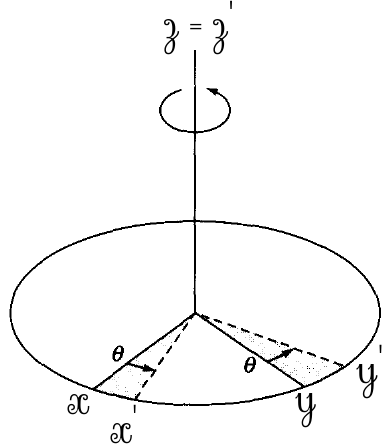
\includegraphics[scale=0.5]{problema2fig1}
 \caption{Rotación del sistema de coordenadas $(x,y,z)$ en dirección de las agujas 
 del reloj sobre el eje $z$ con un ángulo $\theta(t)$.}
 \label{fig:problema2fig1}
\end{figure}

Como el enunciado establece que la partícula está totalmente libre en el espacio
tridimensional, entonces esto quiere decir que no está sujeta a ningún potencial, 
por lo tanto la lagrangiana para el sistema no primado será

\begin{equation}
 L = \frac{1}{2}m (\dot{x}^2 + \dot{y}^2 + \dot{z}^2).
\end{equation}

Por otra parte, la matriz de rotación será 

\begin{equation}
 \lambda = \begin{pmatrix}
          \cos{\theta} & \sen{\theta} & 0 \\
          -\sen{\theta} & \cos{\theta} & 0 \\
          0 & 0 & 1
          \end{pmatrix}
\end{equation}

Por lo tanto tendremos las siguientes transformaciones entre los sistemas, una 
para ir de los primados a los no primados

\begin{align}
 x' &= x\cos{\theta} + y \sen{\theta}, \\
 y' &= -x\sen{\theta} + y\cos{\theta}, \\
 z' &= z,
\end{align}

y una para ir de los no primados a los primados

\begin{align}
 x &= x'\cos{\theta} - y' \sen{\theta}, \\
 y &= x'\sen{\theta} + y'\cos{\theta}, \\
 z &= z',
 \label{eq:transfCoordNonInertial}
\end{align}

Debido a que las necesitaremos en la lagrangiana para el sistema primado, obtengamos 
las primeras derivadas temporales de las ecuaciones \mref{eq:transfCoordNonInertial}

\begin{align}
 \dot{x} &= \dot{x}'\cos{\theta} - x'\dot{\theta}\sen{\theta} - \dot{y}'\sen{\theta} - y'\dot{\theta}\cos{\theta}, \\
 \dot{y} &= \dot{x}'\sen{\theta} + x'\dot{\theta}\cos{\theta} + \dot{y}'\cos{\theta} - y'\dot{\theta}\sen{\theta}, \\
 \dot{z} &= \dot{z}'.
 \label{eq:derivTransfNonInertial1}
\end{align}

Si llamamos a $\dot{\theta} = \omega$, a la cual asociamos la velocidad angular de 
la rotación, entonces las ecuaciones \mref{eq:derivTransfNonInertial1} se convierten en

\begin{align}
  \dot{x} &= \dot{x}'\cos{\theta} - \omega x'\sen{\theta} - \dot{y}'\sen{\theta} - \omega y'\cos{\theta}, \\
 \dot{y} &= \dot{x}'\sen{\theta} + \omega x'\cos{\theta} + \dot{y}'\cos{\theta} - \omega y'\sen{\theta}, \\
 \dot{z} &= \dot{z}'.
 \label{eq:derivTransfNonInertial2}
\end{align}

Podemos escribir \mref{eq:derivTransfNonInertial2} de una forma más compacta,

\begin{align}
 \dot{x} &= (\dot{x}' - \omega y')\cos{\theta} - (\dot{y}' + \omega x')\sen{\theta}, \\
 \dot{y} &= (\dot{y}' + \omega x')\cos{\theta} + (\dot{x}' - \omega y')\sen{\theta}, \\
 \dot{z} &= \dot{z}'.
\end{align}

Entonces la lagrangiana en el sistema primado será

\begin{align}
\begin{split}
 L' & = \frac{1}{2}m\{[(\dot{x}' - \omega y')\cos{\theta} - (\dot{y}' + \omega x')\sen{\theta}]^2 \\ 
 &+ [(\dot{y}' + \omega x')\cos{\theta} + (\dot{x}' - \omega y')\sen{\theta}]^2 + (\dot{z}')^2\}.
 \end{split}
\end{align}

Trabajando el álgebra para estos términos tendremos,

\begin{align*}
 L' &= \frac{1}{2}m [(\dot{x}' - \omega y')^2\cos^2{\theta} - \cancel{2(\dot{x}' - \omega y')(\dot{y}' + \omega x')\cos{\theta}\sen{\theta}} \\
    &+ (\dot{y}' + \omega x')^2\sen^2{\theta} + (\dot{y}' + \omega x')^2\cos^2{\theta} \\
    &+ \cancel{2(\dot{x}' - \omega y')(\dot{y}' + \omega x')\cos{\theta}\sen{\theta}} + (\dot{x}' - \omega y')^2\sen^2{\theta} \\
    &+ (\dot{z}')^2].
\end{align*}

\begin{align*}
 L' &= \frac{1}{2}m [(\dot{x}' - \omega y')^2\cos^2{\theta} + (\dot{y}' + \omega x')^2\sen^2{\theta} + (\dot{y}' + \omega x')^2\cos^2{\theta} \\ 
    &+ (\dot{x}' - \omega y')^2\sen^2{\theta} + (\dot{z}')^2 ].
\end{align*}

\begin{equation*}
 L' = \frac{1}{2}m \left[(\dot{x}' - \omega y')^2\cancelto{1}{(\sen^2{\theta} + \cos^2{\theta})} + 
 (\dot{y}' + \omega x')^2\cancelto{1}{(\sen^2{\theta} + \cos^2{\theta})} + (\dot{z}')^2 \right].
\end{equation*}

\begin{equation*}
 L' = \frac{1}{2}m \left[(\dot{x}' - \omega y')^2 + (\dot{y}' + \omega x')^2  + (\dot{z}')^2\right].
\end{equation*}

\begin{equation*}
 L' = \frac{1}{2}m \left[ (\dot{x}')^2 - 2\omega \dot{x}'y' + \omega^2(\dot{y}')^2 + 
 (\dot{y}')^2 + 2\omega\dot{y}'x' + \omega^2(\dot{x}')^2 + (\dot{z}')^2 \right].
\end{equation*}

\begin{equation}
 \boxed{L' = \frac{1}{2}m \left[ (\dot{x}')^2 + (\dot{y}')^2 + (\dot{z}')^2 + 2\omega(\dot{y}'x' - \dot{x}'y')
 + \omega^2((\dot{y}')^2 + (\dot{x}')^2)\right]. }
\end{equation}

Ahora que hemos encontrado la lagrangiana para el sistema primado podemos utilizar 
las ecuaciones de Lagrange para hallar las expresiones para las fuerzas ficticias 
solicitadas. Recordando que las ecuaciones de Lagrange pueden escribirse, para el 
sistema primado, como

\begin{equation}
 \frac{d}{dt}\frac{\partial L'}{\partial \dot{q}^{i}{'}} - \frac{\partial L'}{\partial q^{i}{'}} = 0
\end{equation}

Tendremos entonces las siguientes ecuaciones de movimiento:

\vspace{.3cm}

Para $x'$,

\begin{align*}
 \frac{d}{dt}(m\dot{x}' - m\omega y') - m\omega\dot{y}' - m\omega^2x' = 0, \\
 %
 m\ddot{x}' - m\omega\dot{y}' - m\dot{\omega}y' - m\omega\dot{y}' - m\omega^2x' = 0,
\end{align*}

\begin{equation}
 \boxed{m\ddot{x}' = 2m\omega\dot{y}' + m\omega^2 x'+ m\dot{\omega}y'}.
 \label{eq:ecuMoviXNonInertial}
\end{equation}

Para $y'$,

\begin{align*}
 \frac{d}{dt}(m\dot{y}' + m\omega x') + m\omega \dot{x}' - m\omega^2y' = 0, \\
 m\ddot{y}' + m\omega\dot{x}' + m\dot{\omega}x' + m\omega \dot{x}' - m\omega^2y' = 0.
\end{align*}

\begin{equation}
 \boxed{m\ddot{y}' = -2m\omega\dot{x}' + m\omega^2 y' - m\dot{\omega}x'.}
  \label{eq:ecuMoviYNonInertial}
\end{equation}

Y para $z'$

\begin{equation}
 \boxed{\frac{d}{dt}(m\dot{z}') = 0 \Rightarrow m\dot{z}' = \text{constante}}
  \label{eq:ecuMoviZNonInertial}
\end{equation}

Podemos ahora fácilmente reconocer las fuerzas ficticias que también se encuentran en 
el tratamiento de sistemas no inerciales con la mecánica vectorial. Los términos 
proporcionales a $\omega$ son las "fuerzas de Coriolis``

\begin{equation}
\boxed{ \vec{F}' \text{(Coriolis)} = (2m\omega\dot{y}', -2m\omega\dot{x}', 0) = -2m\vec{\omega} \times \dot{\vec{r}'}.}
\end{equation}

Los términos proporcionales a $\omega^2$ son las ''fuerzas centrífugas`` 

\begin{equation}
 \boxed{\vec{F}' \text{(Centrífuga)} = ( m \omega^2 x', m\omega^2 y', 0) = - m \vec{\omega} \times (\vec{\omega} \times \vec{r}').}
\end{equation}

Y los términos proporcionales a $\dot{\omega}$ son las ''fuerzas de Euler``

\begin{equation}
 \boxed{\vec{F}' \text{(Euler)} = (m\dot{\omega}y', -m\dot{\omega}x', 0 ) = - m \dot{\vec{\omega}} \times \vec{r}'.}
\end{equation}

Con lo cual hemos comprobado que podemos llegar a las mismas expresiones para las fuerzas 
ficticias desde un marco lagrangiano a las que se encuentran con la mecánica vectorial, pero 
con mucho menos trabajo. Cabe destacar que las fuerzas de Euler surgen debido a que 
hemos considerado que la velocidad angular de rotación puede cambiar en el tiempo.


\section{Problema 3}

Un girocompás es un instrumento que consisten de un cuerpo rígido simétrico, 
$(I_1 = I_2 \ne I_3)$ cuyo eje de simetría está constreñido a permanecer sobre 
un plano horizontal en la superficie de la Tierra, la que, naturalmente está en 
rotación en torno a su eje con un período de 24 horas. Suponga que un girocompás 
se encuentra en un punto de la Tierra de latitud $\phi$ y se pone, inicialmente, 
en rotación en torno a su eje de simetría con una velocidad angular $\omega_3$ cuando 
dicho eje apunta en una dirección arbitraria. Calcule una lagrangiana para este 
sistema. Demuestre que la velocidad de rotación en torno al eje de simetría, $\omega_3$,
permanece constante. Demuestre que si $\omega_3 > (I_1/I_3)\omega_0\cos{\phi}$ entonces 
el eje de simetría oscilará, de manera estable, en torno a la dirección norte-sur 
($\omega_0$ es la velocidad angular de la Tierra).

\vspace{.3cm}

\underline{Solución:} \vspace{.3cm}


\end{document}
